% Preamble templated from Dhawal24112006/EE1030
\documentclass{beamer}
\mode<presentation>
\usepackage{amsmath}
\usepackage{amssymb}
%\usepackage{advdate}
\usepackage{adjustbox}
\usepackage{subcaption}
% \usepackage{enumitem}
\usepackage{multicol}
\usepackage{mathtools}
\usepackage{listings}
\usepackage{url}
\def\UrlBreaks{\do\/\do-}
\usetheme{Boadilla}
\usecolortheme{lily}
\setbeamertemplate{footline}
{
  \leavevmode%
  \hbox{%
  \begin{beamercolorbox}[wd=\paperwidth,ht=2.25ex,dp=1ex,right]{author in head/foot}%
    \insertframenumber{} / \inserttotalframenumber\hspace*{2ex}
  \end{beamercolorbox}}%
  \vskip0pt%
}
\setbeamertemplate{navigation symbols}{}

\providecommand{\nCr}[2]{\,^{#1}C_{#2}} % nCr
\providecommand{\nPr}[2]{\,^{#1}P_{#2}} % nPr
\providecommand{\mbf}{\mathbf}
\providecommand{\pr}[1]{\ensuremath{\Pr\left(#1\right)}}
\providecommand{\qfunc}[1]{\ensuremath{Q\left(#1\right)}}
\providecommand{\sbrak}[1]{\ensuremath{{}\left[#1\right]}}
\providecommand{\lsbrak}[1]{\ensuremath{{}\left[#1\right.}}
\providecommand{\rsbrak}[1]{\ensuremath{{}\left.#1\right]}}
\providecommand{\brak}[1]{\ensuremath{\left(#1\right)}}
\providecommand{\lbrak}[1]{\ensuremath{\left(#1\right.}}
\providecommand{\rbrak}[1]{\ensuremath{\left.#1\right)}}
\providecommand{\cbrak}[1]{\ensuremath{\left\{#1\right\}}}
\providecommand{\lcbrak}[1]{\ensuremath{\left\{#1\right.}}
\providecommand{\rcbrak}[1]{\ensuremath{\left.#1\right\}}}
\theoremstyle{remark}
\newtheorem{rem}{Remark}
\newcommand{\sgn}{\mathop{\mathrm{sgn}}}
\providecommand{\abs}[1]{\left\vert#1\right\vert}
\providecommand{\res}[1]{\Res\displaylimits_{#1}}
\providecommand{\norm}[1]{\lVert#1\rVert}
\providecommand{\mtx}[1]{\mathbf{#1}}
\providecommand{\mean}[1]{E\left[ #1 \right]}
\providecommand{\fourier}{\overset{\mathcal{F}}{ \rightleftharpoons}}
%\providecommand{\hilbert}{\overset{\mathcal{H}}{ \rightleftharpoons}}
\providecommand{\system}{\overset{\mathcal{H}}{ \longleftrightarrow}}
	%\newcommand{\solution}[2]{\textbf{Solution:}{#1}}
%\newcommand{\solution}{\noindent \textbf{Solution: }}
\providecommand{\dec}[2]{\ensuremath{\overset{#1}{\underset{#2}{\gtrless}}}}
\newcommand{\myvec}[1]{\ensuremath{\begin{pmatrix}#1\end{pmatrix}}}
\newcommand{\augvec}[3]{\ensuremath{\begin{amatrix}{#1|#2}#3\end{amatrix}}}
\NewDocumentEnvironment{amatrix}{>{\SplitArgument{1}{|}}m}
 {\left(\makeamatrix#1}
 {\end{array}\right)}
\NewDocumentCommand{\makeamatrix}{mm}{%
  \IfNoValueTF{#2}
    {\begin{array}{@{}*{#1}{c}@{}}}
    {\begin{array}{@{}*{#1}{c}|*{#2}{c}@{}}}%
}
\let\vec\mathbf

\lstset{
%language=C,
frame=single,
breaklines=true,
columns=fullflexible,
showstringspaces=false
}

\numberwithin{equation}{section}

\title{MATGEO Presentation: 4.13.59}
\author{Subhodeep Chakraborty \\ ee25btech11055,\\IIT Hyderabad.}

\date{\today}
\begin{document}

\begin{frame}
\titlepage
\end{frame}

\section*{Outline}
\begin{frame}
\tableofcontents
\end{frame}

\section{Problem}
\begin{frame}
\frametitle{Problem Statement}

Determine all values of $\alpha$ for which the point \brak{\alpha,\alpha^2} lies inside the triangle formed by the lines. \hfill\brak{1992}
\begin{align}
 2x+3y-1&=0\\
 x+2y-3&=0\\
 5x-6y-1&=0
\end{align}
\end{frame}

\section{Solution}
\begin{frame}{Given data}
Given:
\begin{align}
 \vec{n_1}^\top\vec{x}&=c_1 &\vec{n_1}=\myvec{2\\3} c_1 = 1 \\
 \vec{n_2}^\top\vec{x}&=c_2 &\vec{n_2}=\myvec{1\\2} c_2 = 3 \\
 \vec{n_3}^\top\vec{x}&=c_3 &\vec{n_3}=\myvec{5\\-6} c_3 = 1 \\
 \vec{P} &= \myvec{\alpha \\ \alpha^2} &
\end{align}
\end{frame}

\begin{frame}{Formulae}
For finding vertices:
\begin{align}
 \myvec{n_1 & n_2}^\top\vec{V_3} = \myvec{c1 \\ c2} \\
 \myvec{n_3 & n_1}^\top\vec{V_2} = \myvec{c3 \\ c1} \\
 \myvec{n_2 & n_3}^\top\vec{V_1} = \myvec{c2 \\ c3}
\end{align}
Let us define $d_i = \vec{n_i}^\top\vec{V_i}-c_i$ as the sign denoting which side of the line the vertex opposite to it lies on. Also define matrix $\vec{D} = \text{diag}\brak{d_1,d_2,d_3}$ \par\noindent
For point to lie inside triangle, we need $d_i\cdot\brak{\vec{n_i}^\top\vec{P}-c_i} > 0$. In matrix form, this is written as:
\end{frame}
\begin{frame}
\begin{align}
\vec{D} &= \myvec{d_1 & 0 & 0 \\ 0 & d_2 & 0 \\ 0 & 0 & d_3} \\
  &\vec{D}\myvec{\vec{n_1}^\top\vec{P}-c_1 \\ \vec{n_2}^\top\vec{P}-c_2 \\ \vec{n_3}^\top\vec{P}-c_3} > \vec{0}
\end{align}
Let
\begin{align}
 \vec{N} &= \myvec{n_1 & n_2 & n_3}^\top \\
 \vec{C} &= \myvec{c_1 \\ c_2 \\ c_3}
\end{align}
Thus representing everything in terms of matrices,
\begin{align}
 \vec{D}\brak{\vec{N}\vec{P}-\vec{C}} > \vec{0}
\end{align}
is the required inequality.
\end{frame}

\begin{frame}{Solving}
\text{First, we find the vertices of the triangle using Gaussian elimination:}
\begin{align}
 \vec{V_1} :& \augvec{2}{1}{ 1 & 2 & 3 \\ 5 & -6 & 1 } \xrightarrow{R_2 \to R_2 - 5R_1} \augvec{2}{1}{ 1 & 2 & 3 \\ 0 & -16 & -14} \implies \vec{V_1} = \myvec{5/4 \\ 7/8} \\
 \vec{V_2} :& \augvec{2}{1}{ 2 & 3 & 1 \\ 5 & -6 & 1} \xrightarrow{R_2 \to R_2 - \frac{5}{2}R_1} \augvec{2}{1}{ 2 & 3 & 1 \\ 0 & -27/2 & -3/2 } \implies \vec{V_2} = \myvec{1/3 \\ 1/9} \\
 \vec{V_3}:& \augvec{2}{1}{ 2 & 3 & 1 \\ 1 & 2 & 3} \xrightarrow{R_2 \to R_2 - \frac{1}{2}R_1} \augvec{2}{1}{ 2 & 3 & 1 \\ 0 & 1/2 & 5/2 } \implies \vec{V_3} = \myvec{-7 \\ 5}
\end{align}
\end{frame}
\begin{frame}
 \text{Next, we determine the signs } $d_i = \vec{n_i}^\top\vec{V_i}-c_i$ \text{ for each line evaluated at its opposite vertex:}
\begin{align}
 d_1 &= \vec{n_1}^\top\vec{V_1}-c_1 = 2(5/4) + 3(7/8) - 1 = 33/8 \\
 d_2 &= \vec{n_2}^\top\vec{V_2}-c_2 = (1/3) + 2(1/9) - 3 = -22/9 \\
 d_3 &= \vec{n_3}^\top\vec{V_3}-c_3 = 5(-7) - 6(5) - 1 = -66
\end{align}
\text{For the point } $\vec{P} = \myvec{\alpha \\ \alpha^2}$ \text{ to be inside, the condition } $\vec{D}(\vec{N}\vec{P}-\vec{C}) > \vec{0}$ \text{ must hold.}
\begin{align}
 \vec{N}\vec{P}-\vec{C} &= \myvec{2 & 3 \\ 1 & 2 \\ 5 & -6} \myvec{\alpha \\ \alpha^2} - \myvec{1 \\ 3 \\ 1} = \myvec{3\alpha^2+2\alpha-1 \\ 2\alpha^2+\alpha-3 \\ -6\alpha^2+5\alpha-1}
\end{align}
\end{frame}
\begin{frame}
 \text{Multiplying by the diagonal matrix} $\vec{D}$:
\begin{align}
 \vec{D}(\vec{N}\vec{P}-\vec{C}) &= \myvec{33/8 & 0 & 0 \\ 0 & -22/9 & 0 \\ 0 & 0 & -66} \myvec{3\alpha^2+2\alpha-1 \\ 2\alpha^2+\alpha-3 \\ -6\alpha^2+5\alpha-1} \\
 &= \myvec{(33/8)(3\alpha^2+2\alpha-1) \\ (-22/9)(2\alpha^2+\alpha-3) \\ (-66)(-6\alpha^2+5\alpha-1)} > \myvec{0 \\ 0 \\ 0}
\end{align}
\text{This yields the system of inequalities:}
\begin{align}
 3\alpha^2+2\alpha-1 &> 0 \implies \alpha \in \brak{-\infty, -1} \cup \brak{1/3, \infty} \\
 2\alpha^2+\alpha-3 &< 0 \implies \alpha \in \brak{-3/2, 1} \\
 6\alpha^2-5\alpha+1 &> 0 \implies \alpha \in \brak{-\infty, 1/3} \cup \brak{1/2, \infty}
\end{align}
\end{frame}
\begin{frame}{Result}
 \text{The value of } $\alpha$ \text{ must satisfy all three conditions. Taking the intersection of the solution sets:}
\begin{align}
 \alpha \in \brak{-3/2,-1} \cup \brak{1/2, 1}
\end{align}
\end{frame}
\subsection{Plot}
\begin{frame}{Plot}
 \begin{figure}[H]
    \centering
    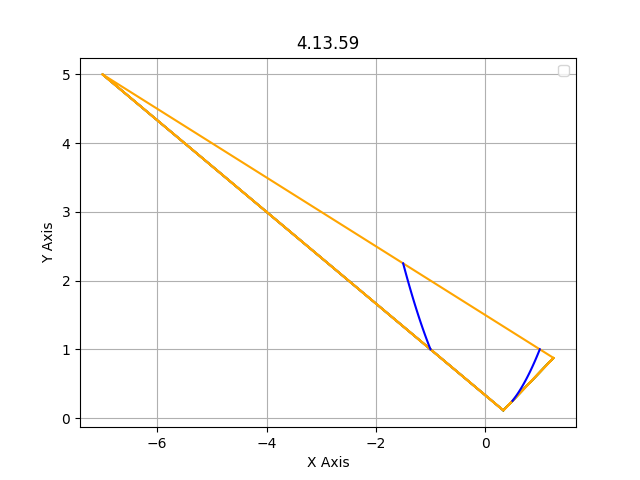
\includegraphics[width=0.8\columnwidth]{../figs/plot.png}
    \caption*{}
    \label{fig:plot}
\end{figure}
\end{frame}

\section{C Code}
\begin{frame}[fragile]{C code for generating points on line}
\begin{lstlisting}[language=C]
 void point_gen(const double* P1, const double* P2, double t, double* result_point) {
    result_point[0] = P1[0] + t * (P2[0] - P1[0]);
    result_point[1] = P1[1] + t * (P2[1] - P1[1]);
    result_point[2] = P1[2] + t * (P2[2] - P1[2]);
}
\end{lstlisting}
\end{frame}

\section{Python Code}
\subsection{Using shared objects}
\begin{frame}[fragile]{Python code for plotting using C}
\begin{lstlisting}[language=Python]
import ctypes
import numpy as np
import numpy.linalg as LA
import matplotlib.pyplot as plt
from mpl_toolkits.mplot3d import Axes3D

libline = ctypes.CDLL("./line.so")

get_point = libline.point_gen
get_point.argtypes = [
    ctypes.POINTER(ctypes.c_double),  # P1
    ctypes.POINTER(ctypes.c_double),  # P2
    ctypes.c_double,  # t
    ctypes.POINTER(ctypes.c_double),  # result_point
]
get_point.restype = None
\end{lstlisting}
\end{frame}
\begin{frame}[fragile]
 \begin{lstlisting}[language=Python]
DoubleArray3 = ctypes.c_double * 3
a = DoubleArray3(5, 1, 6)
b = DoubleArray3(3, 4, 1)
c = DoubleArray3(13 / 5, 23 / 5, 0)

fig = plt.figure(figsize=(8, 6))
ax = fig.add_subplot(111, projection="3d")

t_values = np.linspace(0, 1, 100)
line_points_x, line_points_y, line_points_z = [], [], []

for t in t_values:
    result_arr = DoubleArray3()

    get_point(a, c, t, result_arr)

    line_points_x.append(result_arr[0])
    line_points_y.append(result_arr[1])
    line_points_z.append(result_arr[2])
 \end{lstlisting}
\end{frame}
\begin{frame}[fragile]
 \begin{lstlisting}[language=Python]
ax.plot(
    line_points_x,
    line_points_y,
    line_points_z,
    color="gray",
)
ax.scatter(b[0], b[1], b[2], color="blue", label="b")
ax.scatter(a[0], a[1], a[2], color="red", label="a")
ax.scatter(c[0], c[1], c[2], color="green", label="Point")

ax.set_xlabel("X Axis")
ax.set_ylabel("Y Axis")
ax.set_zlabel("Z Axis")
ax.set_title("2.9.6")
ax.legend()
ax.grid(True)
plt.savefig("../figs/plot.png")
plt.show()
 \end{lstlisting}
\end{frame}
\subsection{Plot}
\begin{frame}{Plot}
 \begin{figure}[H]
    \centering
    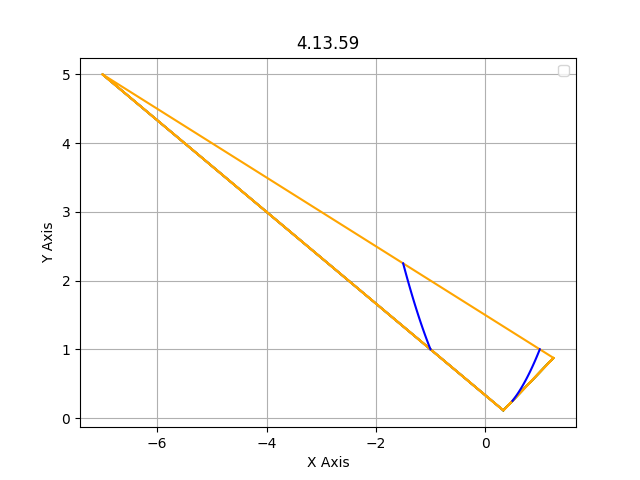
\includegraphics[width=0.8\columnwidth]{../figs/plot.png}
    \caption*{}
    \label{fig:plot}
\end{figure}
\end{frame}
\subsection{In pure Python}
\begin{frame}[fragile]{Pure Python code}
 \begin{lstlisting}[language=Python]
import numpy as np
import matplotlib.pyplot as plt
from mpl_toolkits.mplot3d import Axes3D

a = np.array([5, 1, 6]).T
b = np.array([3, 4, 1]).T
c = np.array([13 / 5, 23 / 5, 0])

fig = plt.figure(figsize=(8, 8))
ax = fig.add_subplot(111, projection="3d")

ax.plot([a[0], c[0]], [a[1], c[1]], [a[2], c[2]], color="blue", label="b")

ax.scatter(b[0], b[1], b[2], color="blue", label="b")
ax.scatter(a[0], a[1], a[2], color="red", label="a")
ax.scatter(c[0], c[1], c[2], color="green", label="Point")
 \end{lstlisting}
\end{frame}
\begin{frame}[fragile]{Pure Python code}
 \begin{lstlisting}[language=Python]
ax.text(a[0], a[1], a[2], "A")
ax.text(b[0], b[1], b[2], "B")
ax.text(c[0], c[1], c[2], "Point")

ax.set_xlabel("X-axis")
ax.set_ylabel("Y-axis")
ax.set_zlabel("Z-axis")
ax.set_title("2.9.6")
ax.set_xlim([-5, 5])
ax.set_ylim([-5, 5])
ax.set_zlim([-5, 5])
ax.legend()
ax.grid(True)

plt.savefig("../figs/python.png")
plt.show()
 \end{lstlisting}
\end{frame}
\subsection{Plot}
\begin{frame}{Plot}
 \begin{figure}[H]
    \centering
    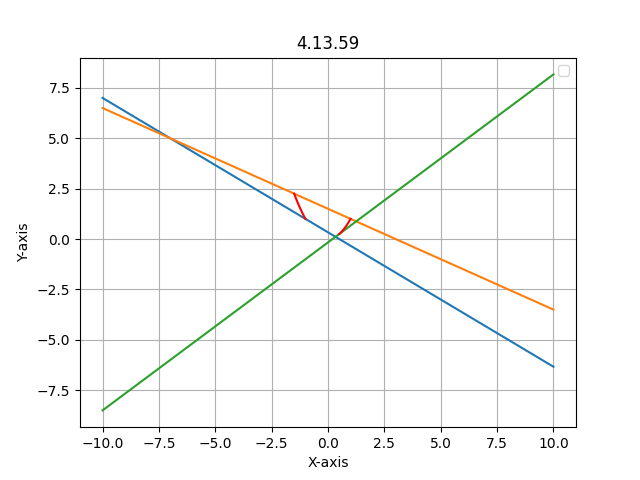
\includegraphics[width=0.75\columnwidth]{../figs/python.png}
    \caption*{}
    \label{fig:plot}
\end{figure}
\end{frame}
\end{document}
